% ------------------------------------------------------------------------------
% TYPO3 Version 10.3 - What's New (French Version)
%
% @license	Creative Commons BY-NC-SA 3.0
% @link		https://typo3.org/help/documentation/whats-new/
% @language	French
% ------------------------------------------------------------------------------

\section{Changements pour les développeurs}
\begin{frame}[fragile]
	\frametitle{Changements pour les développeurs}

	\begin{center}\huge{Chapitre 3~:}\end{center}
	\begin{center}\huge{\color{typo3darkgrey}\textbf{Changements pour les développeurs}}\end{center}

\end{frame}

% ------------------------------------------------------------------------------
% Feature | 90333 | Dashboard

\begin{frame}[fragile]
	\frametitle{Changements pour les développeurs}
	\framesubtitle{Tableau de bord (1)}

	% decrease font size for code listing
	\lstset{basicstyle=\smaller\ttfamily}

	\begin{itemize}
		\item Les développeurs peuvent créer des widgets pour le tableau de
			bord en se basant sur l'une de ces base de widget~:

			\begin{itemize}
				\item \texttt{AbstractWidget}\newline
					\small
						Une base pouvant être utilisée pour démarrer un widget simple.
					\normalsize
				\item \texttt{AbstractRssWidget}\newline
					\small
						Une base pour créer un widget affichant un flux RSS.
					\normalsize
				\item \texttt{AbstractListWidget}\newline
					\small
						Une base pour créer un widget affichant une liste.
					\normalsize
				\item \texttt{AbstractCtaButtonWidget}\newline
					\small
						Une base pour créer un widget qui affiche un bouton d'action.
					\normalsize
			\end{itemize}

	\end{itemize}

\end{frame}

% ------------------------------------------------------------------------------
% Feature | 90333 | Dashboard

\begin{frame}[fragile]
	\frametitle{Changements pour les développeurs}
	\framesubtitle{Tableau de bord (2)}

	% decrease font size for code listing
	\lstset{basicstyle=\tiny\ttfamily}

	\begin{itemize}
		\item L'inscription des widget s'effectue dans le fichier suivant des extensions~:\newline
			\texttt{EXT:my\_extension/Configuration/Services.yaml}

		\item Option 1~: identifiant du widget en attribut

\vspace{-0.4cm}
\begin{lstlisting}
Vendor\MyExtension\Widgets\MyFirstWidget:
  tags:
    - name: dashboard.widget
      identifier: widget-identifier-1
      widgetGroups: 'general'
\end{lstlisting}

		\item Option 2~: service personnalisé permettant de définir plusieurs widget
			dans une seule classe

\vspace{-0.4cm}
\begin{lstlisting}
widget.identifier:
  class: Vendor\MyExtension\Widgets\MySecondWidget
  tags:
    - name: dashboard.widget
      identifier: widget-identifier-2
      widgetGroups: 'general, typo3'
\end{lstlisting}

	\end{itemize}

\end{frame}

% ------------------------------------------------------------------------------
% Feature | 90333 | Dashboard

\begin{frame}[fragile]
	\frametitle{Changements pour les développeurs}
	\framesubtitle{Tableau de bord (3)}

	% decrease font size for code listing
	\lstset{basicstyle=\tiny\ttfamily}

	\begin{itemize}
		\item Chaque widget est attaché à un ou plieurs groupes.
		\item Ces groupes sont affichés dans la boîte de dialogue lors de l'ajout
			d'un widget au tableau de bord.
		\item Les développeurs peuvent définir des groupes de widget dans le fichier\newline
			\smaller
				\texttt{EXT:my\_extension/Configuration/Backend/DashboardWidgetGroups.php}
			\normalsize

\vspace{-0.4cm}
\begin{lstlisting}
return [
  'widgetGroup-exampleGroup' => [
    'title' => 'LLL:EXT:my_extension/Resources/Private/Language/locallang.xlf:widget_group_name',
  ],
];
\end{lstlisting}

	\end{itemize}

\end{frame}

% ------------------------------------------------------------------------------
% Feature | 89870 | New PSR-14 Events for Extbase-related signals

\begin{frame}[fragile]
	\frametitle{Changements pour les développeurs}
	\framesubtitle{Extbase et Fluid}

	% decrease font size for code listing
	\lstset{basicstyle=\tiny\ttfamily}

	\begin{itemize}
		\item Les événements suivants basés sur PSR-14 sont introduits pour des signaux Extbase~:

\vspace{-0.4cm}
\begin{lstlisting}
TYPO3\CMS\Extbase\Event\Mvc\AfterRequestDispatchedEvent
TYPO3\CMS\Extbase\Event\Mvc\BeforeActionCallEvent
TYPO3\CMS\Extbase\Event\Persistence\AfterObjectThawedEvent
TYPO3\CMS\Extbase\Event\Persistence\ModifyQueryBeforeFetchingObjectDataEvent
TYPO3\CMS\Extbase\Event\Persistence\ModifyResultAfterFetchingObjectDataEvent
TYPO3\CMS\Extbase\Event\Persistence\EntityAddedToPersistenceEvent
TYPO3\CMS\Extbase\Event\Persistence\EntityFinalizedAfterPersistenceEvent
TYPO3\CMS\Extbase\Event\Persistence\EntityUpdatedInPersistenceEvent
TYPO3\CMS\Extbase\Event\Persistence\EntityRemovedFromPersistenceEvent
TYPO3\CMS\Extbase\Event\Persistence\EntityPersistedEvent
\end{lstlisting}

		\item Les signaux existants sont remplacés et ne doivent plus être utilisés.

	\end{itemize}

\end{frame}

% ------------------------------------------------------------------------------
% Feature | 89644 | Add optional argument fields to editRecord ViewHelpers

\begin{frame}[fragile]
	\frametitle{Changements pour les développeurs}
	\framesubtitle{ViewHelper \texttt{editRecord}}

	% decrease font size for code listing
	\lstset{basicstyle=\tiny\ttfamily}

	\begin{itemize}
		\item L'argument optionnel \texttt{fields} est ajouté aux ViewHelpers
			\texttt{uri.editRecord} et \texttt{link.editRecord}.
		\item Si défini, le moteur de formulaire créé un formulaire pour éditer
			uniquement les champs spécifiés
		\item L'exemple suivant génère un lien pour éditer le champs \texttt{tt\_content.bodytext}
			de l'enregistrement avec l'identifiant 42.

\begin{lstlisting}
<be:link.editRecord uid="42" table="tt_content" fields="bodytext" returnUrl="foo/bar">
  Edit record
</be:link.editRecord>
\end{lstlisting}

	\end{itemize}

\end{frame}

% ------------------------------------------------------------------------------
% Feature | xxxxx | Introduce AssetCollector

\begin{frame}[fragile]
	\frametitle{Changements pour les développeurs}
	\framesubtitle{AssetCollector}

	\begin{itemize}
		\item Les étapes initiales pour intégrer un collecteur de ressources sont commencées.
		\item Ce concept permet aux développeurs d'ajouter du code CSS/JS (direct ou externe)
			plusieurs fois, mais TYPO3 les renvoient tous en même temps.
		\item À cet égard, deux ViewHelpers Fluid sont ajoutés~:
			\begin{itemize}
				\item \texttt{<f:asset.css>}
				\item \texttt{<f:asset.script>}
			\end{itemize}
		\item À terme, l'usage du collecteur vise à remplacer les options TypoScript
			variées existantes qui sont confusantes.
	\end{itemize}

\end{frame}

% ------------------------------------------------------------------------------
% Feature | 86614 | Add PSR-14 event to control hreflang tags to be rendered

\begin{frame}[fragile]
	\frametitle{Changements pour les développeurs}
	\framesubtitle{Modifier les balises \texttt{hreflang}}

	% decrease font size for code listing
	\lstset{basicstyle=\smaller\ttfamily}

	\begin{itemize}
		\item Il est possible d'altérer les balises \texttt{hreflang} avant qu'elles soient transmises.
		\item Il faut inscrire un écouteur à l'événement suivant~:\newline
			\smaller
				\texttt{TYPO3\textbackslash
					CMS\textbackslash
					Frontend\textbackslash
					Event\textbackslash
					ModifyHrefLangTagsEvent}
			\normalsize
	\end{itemize}

\end{frame}

% ------------------------------------------------------------------------------
% Feature | 88818 | Introduce events to modify CKEditor configuration

\begin{frame}[fragile]
	\frametitle{Changements pour les développeurs}
	\framesubtitle{Modifier la configuration de CKEditor}

	% decrease font size for code listing
	\lstset{basicstyle=\tiny\ttfamily}

	\begin{itemize}
		\item Les événements basés sur PSR-14 suivants permettent d'altérer la configuration de CKEditor~:

\vspace{-0.4cm}
\begin{lstlisting}
TYPO3\CMS\RteCKEditor\Form\Element\Event\AfterGetExternalPluginsEvent
TYPO3\CMS\RteCKEditor\Form\Element\Event\BeforeGetExternalPluginsEvent
TYPO3\CMS\RteCKEditor\Form\Element\Event\AfterPrepareConfigurationForEditorEvent
TYPO3\CMS\RteCKEditor\Form\Element\Event\BeforePrepareConfigurationForEditorEvent
\end{lstlisting}

		\item Voir le
			\href{https://docs.typo3.org/c/typo3/cms-core/master/en-us/Changelog/10.3/Feature-88818-IntroduceEventsToModifyCKEditorConfiguration.html}{journal des modifications (en)}
			pour un exemple.
	\end{itemize}

\end{frame}

% ------------------------------------------------------------------------------
% Feature | 90265 | Show dispatched Events in Admin Panel

\begin{frame}[fragile]
	\frametitle{Changements pour les développeurs}
	\framesubtitle{Événements PSR-14 dans le panneau d'administration}

	\begin{itemize}
		\item Le panneau d'administration affiche tous les événements PSR-14
			qui ont été déclenchés dans la requête courante.
	\end{itemize}

	\begin{figure}
		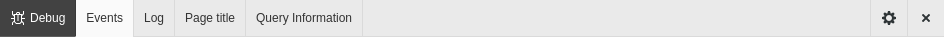
\includegraphics[width=0.85\linewidth]{ChangesForDevelopers/90265-ShowDispatchedEventsInAdminPanel.png}
	\end{figure}

\end{frame}

% ------------------------------------------------------------------------------
% Feature | 89738 | API for AJAX Requests

\begin{frame}[fragile]
	\frametitle{Changements pour les développeurs}
	\framesubtitle{API pour les requêtes AJAX}

	% decrease font size for code listing
	\lstset{basicstyle=\tiny\ttfamily}

	\begin{itemize}
		\item L'API \textbf{Fetch} est introduite pour effectuer des requêtes AJAX
			et pour rendre TYPO3 moins dépendant de jQuery.
		\item L'API fournit une définition générique d'objets Requête et Réponse
			(et d'autres éléments impliqués dans les requêtes réseau)
		\item Supportée par tous les navigateurs modernes, voir le
			\href{https://developer.mozilla.org/en-US/docs/Web/API/Fetch_API}{tableau de compatibilité}.
		\item Le noyau de TYPO3 utilise déjà la nouvelle API dans l'outils d'installation, le moteur de
			formulaire et les menus contextuels.
		\item Voir le
			\href{https://docs.typo3.org/c/typo3/cms-core/master/en-us/Changelog/10.3/Feature-89738-ApiForAjaxRequests.html}{journal des modifications (en)}
			pour des exemples de comment utiliser l'API Fetch.

	\end{itemize}

\end{frame}

% ------------------------------------------------------------------------------
% Feature | 89650 | Allow line breaks in TCA descriptions

\begin{frame}[fragile]
	\frametitle{Changements pour les développeurs}
	\framesubtitle{Champs de description TCA}

	\begin{itemize}
		\item Les sauts de ligne sont acceptés dans les champs de description TCA
			pour rendre les texte longs plus lisibles.
	\end{itemize}

\end{frame}

% ------------------------------------------------------------------------------
% Important | 90020 | Legacy BasicFileUtility and ExtendedFileUtility classes marked as internal

\begin{frame}[fragile]
	\frametitle{Changements pour les développeurs}
	\framesubtitle{Classes \texttt{BasicFileUtility} et \texttt{ExtendedFileUtility}}

	\begin{itemize}
		\item Ces deux anciennes classes sont marquées \textbf{internes}
			et ne doivent plus être utilisées~:

			\begin{itemize}\small
				\item \texttt{TYPO3\textbackslash
					CMS\textbackslash
					Core\textbackslash
					Utility\textbackslash
					File\textbackslash
					BasicFileUtility}
				\item \texttt{TYPO3\textbackslash
					CMS\textbackslash
					Core\textbackslash
					Utility\textbackslash
					File\textbackslash
					ExtendedFileUtility}
			\end{itemize}

		\item Les développeurs doivent utiliser les classes \texttt{ResourceStorage}
			et \texttt{ResourceFactory} pour gérer les fichiers.

	\end{itemize}

\end{frame}

% ------------------------------------------------------------------------------
% Feature | 89139 | Add dependency injection support for console commands

\begin{frame}[fragile]
	\frametitle{Changements pour les développeurs}
	\framesubtitle{Commandes de Console~: Support Symfony DI}

	\begin{itemize}
		\item Les dépendances des commandes peuvent être injectées par le constructeur ou d'autres
			techniques d'injection.
		\item Ajoutez la balise \texttt{console.command} aux classes de commande.
		\item Utilisez la balise d'attribut \texttt{command} pour spécifier le nom de la commande.
		\item Pour exclure la commande du planificateur TYPO3, il faut définir la balise d'attribut
			optionnel \texttt{schedulable} à \texttt{false}.

		\item Voir le
			\href{https://docs.typo3.org/c/typo3/cms-core/master/en-us/Changelog/10.3/Feature-89139-AddDependencyInjectionSupportForConsoleCommands.html}{journal des modifications (en)}
			pour un exemple.
	\end{itemize}

\end{frame}

% ------------------------------------------------------------------------------
% Feature | 90168 | Introduce Modal Actions

\begin{frame}[fragile]
	\frametitle{Changements pour les développeurs}
	\framesubtitle{Boutons d'action dans les boîtes de dialogue}

	% decrease font size for code listing
	\lstset{basicstyle=\tiny\ttfamily}

	\begin{itemize}
		\item Les boîtes de dialogue supportent les boutons d'action.
		\item En alternative à l'option existante \texttt{trigger}, la nouvelle
			option \texttt{action} est disponible.
		\item Par exemple~:

\vspace{-0.4cm}
\begin{lstlisting}
Modal.confirm('Header', 'Some content', Severity.error, [
  {
    text: 'Based on trigger()',
    trigger: function () {
      console.log('Vintage!');
    }
  },
  {
    text: 'Based on action()',
    action: new DeferredAction(() => {
      return new AjaxRequest('/any/endpoint').post({});
    })
  }
]);
\end{lstlisting}

	\end{itemize}

\end{frame}

% ------------------------------------------------------------------------------
% Feature | 90471 | JavaScript Event API

\begin{frame}[fragile]
	\frametitle{Changements pour les développeurs}
	\framesubtitle{API d'événement JavaScript}

	\begin{itemize}
		\item L'API d'Événement JavaScript permet aux développeurs d'avoir une
			interface d'écoute d'événement stable.
		\item L'API prend en charge les écueils habituels comme la délégation
			d'événement et le détachement propre d'événement.
		\item Chaque \textit{event strategy} offre deux manières d'associer un
			écouteur à un événement
		\item L'API d'Événement offres plusieurs stratégies pour gérer les écouteurs.
		\item Voir le
			\href{https://docs.typo3.org/c/typo3/cms-core/master/en-us/Changelog/10.3/Feature-90471-JavaScriptEventAPI.html}{journal des modifications (en)}
			pour des exemples et plus de détails.
	\end{itemize}

\end{frame}

% ------------------------------------------------------------------------------
